\documentclass[../main/main.tex]{subfiles}


\begin{document}

\section{February 17th, 2021}
\subsection{Design of Experimental Study}
\index{random assignment}
In order to ensure eliminate any pre-existing group differences, we perform \vocab{random assignment} to assign the participants to the experimental and control groups.  To do this, we can generate a random number to determine how to assign the participants.

\subsection{Dialogic Reading Study}
One real life example of an experimental study is that of the Whitehurst et al. (1988) dialogic reading study.
\begin{remark}
Dialogic reading means that the child and the adult have a conversation while reading the book, instead of just being read to.
\end{remark}
The study was conducted as follows:
\begin{description}
  \item[Participants:] Middle-class children ages 21 to 35 months and their parents
  \item[Experimental group:] The parents adopted dialogic reading
        \item[Control group:] Parents simply read aloud the story
        \item[Observation:] After 1 month, the parents were tested on their language skills
\end{description}
In this study, the IV is reading method, while the DV is the child's language skills.

\begin{remark}
After 1 month, the children in the experimental group were 8.5 months ahead of the control group in the level of speech and 6 months ahead in vocabulary. 9 months later, the experimental group was still 6 months ahead of the control group.
\end{remark}
  The reason why dialogic reading helped to develop the child's language skill because of \vocab{PEER}.
  \begin{description}
	\item[P:] Prompt - the parent would ask the child about what is in the book
	\item[E:] Evaluate - the parents will evaluate the response
	\item[E:] Expand - the parents will expand on the child's response
	\item[R:] Repeat - the parents would ask the child to repeat afterwards to solidify the expansion
  \end{description}
The active participation allows the child to think and to practice their language skills.

\subsection{Measuring Developmental Change}
To measure developmental changes, there are a few different ways to research changes across a person's lifespan. They are:
\begin{itemize}
\item Cross-sectional research
\item Longitudinal research
\item Sequential research
\end{itemize}

\subsubsection{Cross-Sectional Research}
\begin{definition}
\vocab{Cross-sectional research} is where people from different age groups are studied at the same time point. \index{cross-sectional research}
\end{definition}
One major advantage of cross-sectional research is that it is relatively quick to do. However, it has a few disadvantages, as possible age differences may be due to cohort effect.

\begin{definition} \index{cohort effect}
\vocab{Cohort effect} are  variations among individuals who are defined by some shared temporal experience or common life experience.
\end{definition}
\begin{example}
  Suppose you find that people who are 25 year old perform better than those that are 75 year old in an IQ test. This has two possible explanation:
  \begin{enumerate}
    \item The difference in IQ could be a developmental change.
          \item Could be due to cohort effect since the people who are 25 might have a more formal education.
          \item Could also because of a difference in nutrition when they were infants.
  \end{enumerate}
\end{example}
\begin{remark}
A cohort effect is a confounding variable.
\end{remark}

\begin{figure}[htpb]
  \centering
  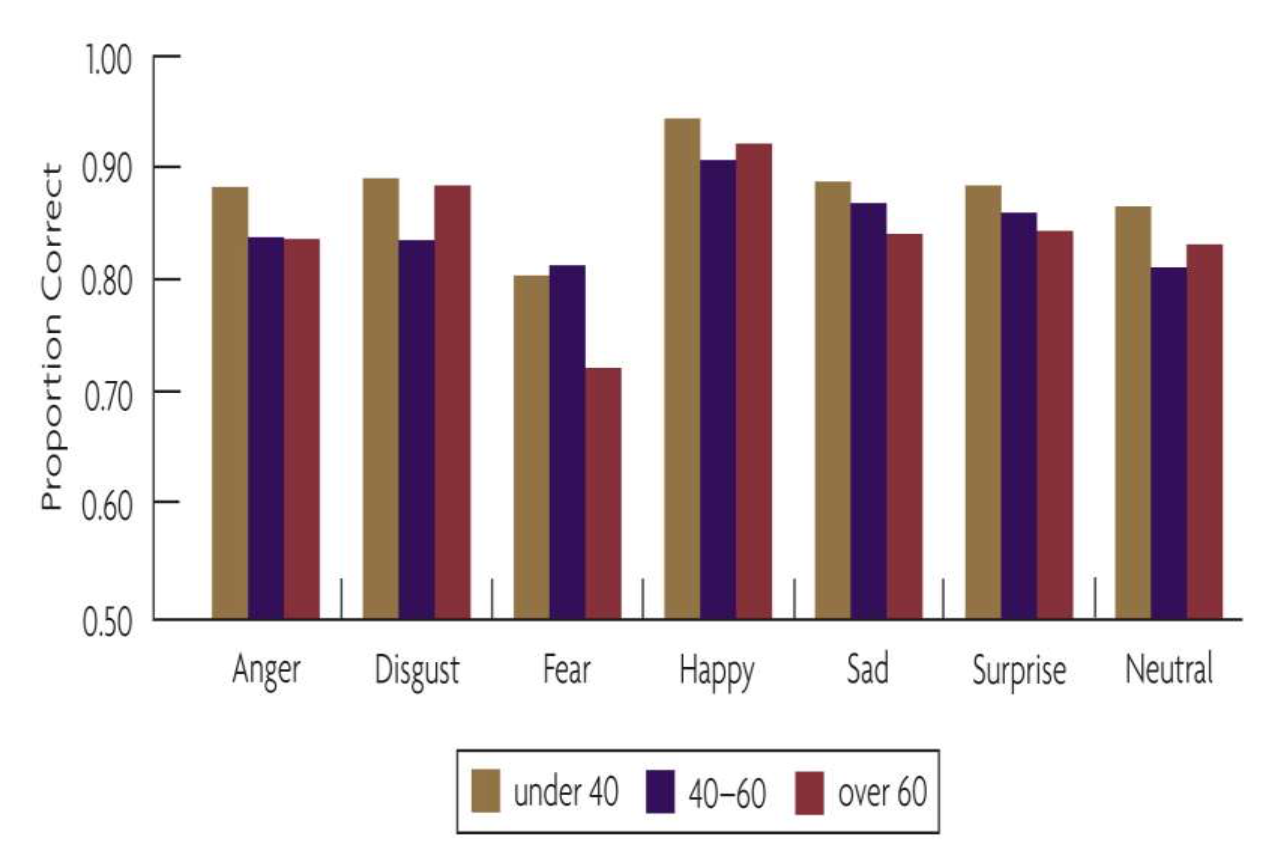
\includegraphics[width=0.6\textwidth]{2-17-ident}
  \caption{Example of a cross-sectional study}
  \label{2-17-ident}
\end{figure}

\begin{example}
  Figure \ref{2-17-ident} shows the result of a  cross-sectional study.
The study investigated the ability to recognize facial expression. Those over 60 performed worse than those who are younger. However, we don't know if this is due to age differences or because of cohort effect (e.g. education).
\end{example}

\subsubsection{Longitudinal Research}

\begin{definition}
In a \vocab{longitudinal research} study, the same group of people is traced over time to assess individual change.
\end{definition}
\begin{example}
Say we took an IQ test now at age 20. Then we take it again at age 70. This is a longitudinal design, as the same group of people are traced over time.
\label{2-17-ex}
\end{example}
\begin{remark}
  The major disadvantage of longitudinal design is because it is time consuming. In Example \ref{2-17-ex}, it would have taken 50 years to perform the study.\\

  In addition, this increases the chance that the participant would drop out of the study, move away, or pass away. This is called an \vocab{attrition problem}. \index{attrition problem} This is an issue, as the samples that remain in the study might be a biased sample. As such, the sample that remain might not be representative of the starting sample, and of course the general population.\\

  Longitudinal design also runs into the problem of the \vocab{practice effect}\index{practice effect}. This is because, if we take the same test over and over, we might perform better because of that.

\end{remark}

\subsubsection{Sequential Reserach}
\begin{definition}
  \index{sequential research}
A \vocab{sequential research} is one where the researchers study a number of different age groups over several points in time.
\end{definition}
\begin{remark}
A sequential design allows researchers to example age change vs. age difference.
\end{remark}
\begin{example}
For example, if we study the moral behavior of children, we might use a sequential design. We might recruit children of age 3, 4, and 5. Then, we would perform the study to these three groups over a period of time.
\end{example}

\begin{figure}[htpb]
  \centering
  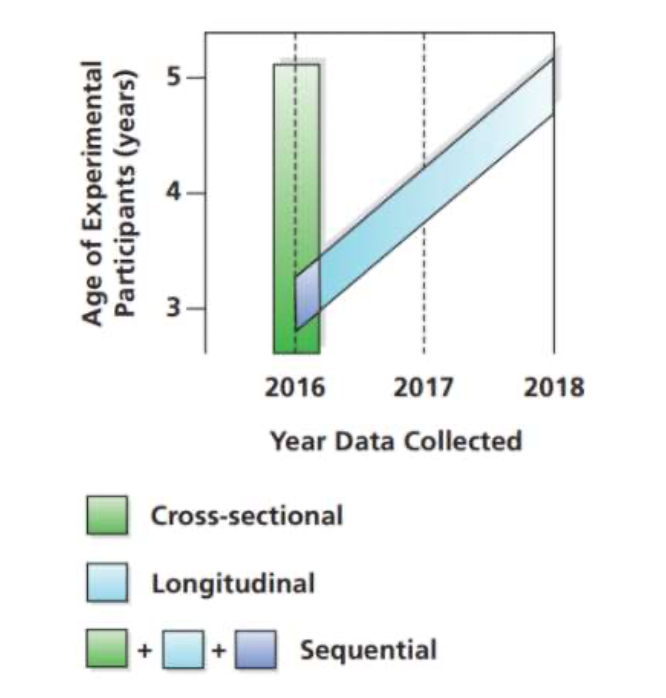
\includegraphics[width=0.5\textwidth]{2-17-seq}
  \caption{Differences between cross-sectional, longitudinal, and sequential design}
\end{figure}

\subsection{Reading - Chapter 1}
//TODO:

\subsection{Theories of Development}
To start, we must define what a theory is. We will then talk about 5 different theoretical perspectives of development:
\begin{enumerate}
\item Psychodynamic perspective
\item Behavioral perspective
\item Cognitive perspective
\item Humanistic perspective
\item Biological perspective
\end{enumerate}

\begin{definition}
A \vocab{theory} refers to the explanations and predictions concerning phenomena of interest. It provides a framework for understanding the relationships among an organized set of facts or principles. \index{theory}
\end{definition}
\begin{remark}
In laymen terms, a theory is a way to explain or predict a phenomenon.
\end{remark}
\begin{example}
Say we want to investigate drug use problems. We might develop theories to explain these phenomenons, for example the observational learning theory. We can then study the correlation or causal relation of this theory. We might also be able to use these theories to predict which teenagers will be more susceptible to drug abuse.
\end{example}

Developmental psychology is similar to the blind men describing the elephant metaphor, where different blind men touching the elephant would describe it differently. Similarly, in developmental psychology, we are looking at different aspects of human development, and thus result in different theories.

\subsection{Psychodynamic Perspective}
\begin{definition}\index{psychodynamic perspective}
  The \vocab{psychodynamic perspective} of developmental psychology says that development is shaped by inner forces, memories, and conflicts.
\end{definition}
There are two main theories from the psychodynamic perspective:
\begin{itemize}
  \item Freud's Psychoanalytic Theory
        \item Erikson’s Psychosocial Theory
\end{itemize}
\subsubsection{Freud's Psychosexual Development Theory}
\index{Freud's psychosexual development theory}
Freud observed a phenomenon (glove anesthesia) in his patients that couldn't be explained by Freud's theory has 3 personality structures:
\begin{itemize}
  \item Id
        \item Ego
        \item Superego
\end{itemize}

\begin{definition}
  \index{id} \index{libido}
The \vocab{id} of a person seeks to maximize \vocab{libido}, which are sexual instincts or aggressive impulses.
\end{definition}
\begin{remark}
Some of these libido are disturbing in nature or not socially acceptable.
\end{remark}
\begin{remark}
  The Id is also called the \vocab{pleasure principle}.
\end{remark}

\begin{definition}
  \index{ego}
  The \vocab{ego} is in charge of gratifying the id that are acceptable to the superego
\end{definition}
\begin{remark}
  The ego is also known as the \index{reality principle}.
\end{remark}
\begin{remark}
We are not born with ego and we develop it when we are around 1 year old.
The majority of the ego functions are conscious to us.
\end{remark}

\begin{definition}
  \index{superego}
The \vocab{superego} acts as the moral judge of the person and tells us what is right or wrong.
\end{definition}
\begin{example}
The superego considers what is socially acceptable or not.
\end{example}
\begin{remark}
We are also not born with the superego, but it is develop at age 5-6 through exposure.
\end{remark}

In this theory, the ego needs to keep the three components in balance, or else tension would occur.

\begin{example}
Say your friend asks you to drink before your exam. The id would tell you to go drink, while the superego would tell you do revise. The ego strikes the balance, e.g. study with a reasonable and realistic timetable.
\end{example}

With these three forces, Freud develop a psychosexual development theory. This theory says that:
\begin{itemize}
        \item Development is fundamentally stage-like, with each stage centered on a particular conflict between sexual urges and demands of society
\item The specific personality a child develops depends on the degree of success the child has in moving through the various stages
\item Over-indulgence (id) or lack of gratification (superego) results in fixation
        \begin{definition}
          \vocab{Fixations} are conflicts or concerns that persist beyond the developmental stage in which they first occur.
        \end{definition}
        \begin{remark}
If the ego is able to develop a good balance, then the person develops a healthy personality.
        \end{remark}
  \item Sequence of stage is determined by maturation
        \begin{itemize}
        \item Unvarying sequence across all individuals
        \end{itemize}
\end{itemize}

This means that during the developmental stage, the ego must strike a good balance between the id and superego. Figure \ref{2-17-5} shows the 5 stages of development according to Freud.
\begin{figure}[htpb]
  \centering
  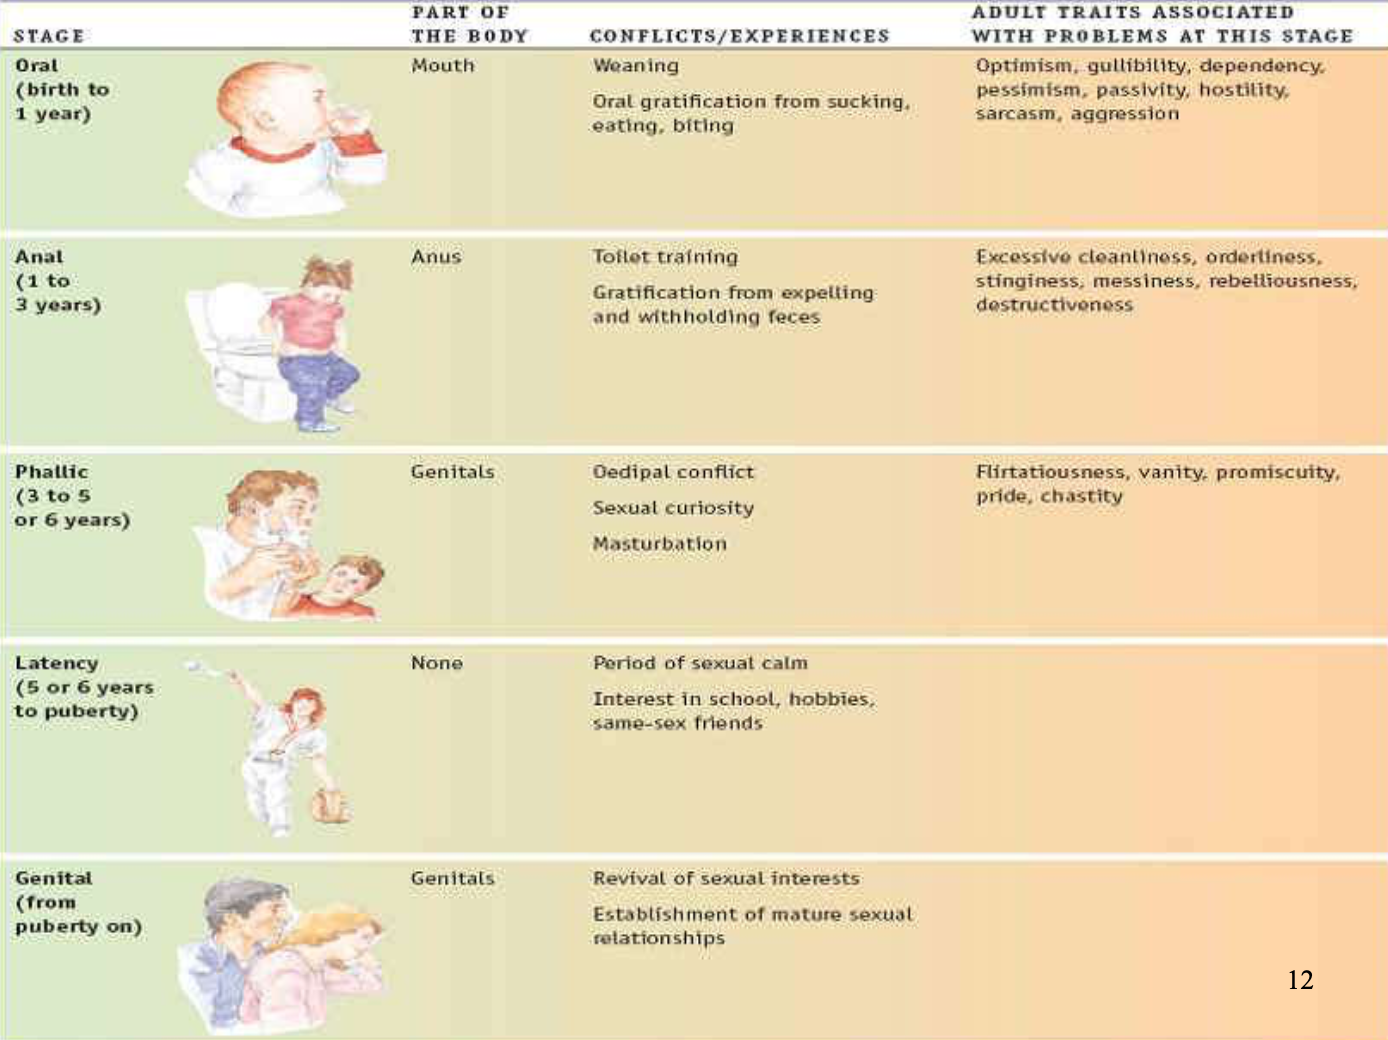
\includegraphics[width=\textwidth]{2-17-5}
  \caption{5 Stages of development according to the Psychosexual theory of development}
  \label{2-17-5}
\end{figure}
\begin{remark}
Freud's theory generally says that human development revolves around our libido and the unconscious forces to gratify these sexual desires. If we are not able to gratify (or over-indulge), we will
\end{remark}
There are quite a few of limitations to Freud's theory:
\begin{itemize}
\item Lack of empirical data and verification (libido is unconscious)
\item Derivation of the concepts and theories from a limited population (only on upper class Austrian women)
\item Freud's theory only considers development until puberty. Development is lifelong and does not stop after adolescence
\item Narrow emphasis on sexual drives and neglect other motives
\end{itemize}
However, Freud's theory did contribute the fact of the importance of unconsciousness in human development.

\end{document}
